%%%%%%%%%%%%%%%%%%%%%%%%%%%%%%%%%%%%%%%%%
% fphw Assignment
% LaTeX Template
% Version 1.0 (27/04/2019)
%
% This template originates from:
% https://www.LaTeXTemplates.com
%
% Authors:
% Class by Felipe Portales-Oliva (f.portales.oliva@gmail.com) with template 
% content and modifications by Vel (vel@LaTeXTemplates.com)
%
% Template (this file) License:
% CC BY-NC-SA 3.0 (http://creativecommons.org/licenses/by-nc-sa/3.0/)
%
%%%%%%%%%%%%%%%%%%%%%%%%%%%%%%%%%%%%%%%%%

%----------------------------------------------------------------------------------------
%	PACKAGES AND OTHER DOCUMENT CONFIGURATIONS
%----------------------------------------------------------------------------------------

\documentclass[
	12pt, % Default font size, values between 10pt-12pt are allowed
	%letterpaper, % Uncomment for US letter paper size
	%spanish, % Uncomment for Spanish
]{fphw}
\usepackage{subcaption}
% Template-specific packages
\usepackage[utf8]{inputenc} % Required for inputting international characters
\usepackage[T1]{fontenc} % Output font encoding for international characters
\usepackage{mathpazo} % Use the Palatino font
\usepackage{amsmath}
\usepackage{tikz}
\usepackage{graphicx} % Required for including images
\usepackage{hyperref}
\usepackage{booktabs} % Required for better horizontal rules in tables
\usepackage{listings} % Required for insertion of code
\usepackage{enumerate} % To modify the enumerate environment
\usepackage{bbm}% from mathbbm.sty
\usepackage{array}
%----------------------------------------------------------------------------------------
%	ASSIGNMENT INFORMATION
%----------------------------------------------------------------------------------------

\title{Homework \#3} % Assignment title

\author{Fanyi Meng (223015127)} % Student name

\date{March 31st, 2024} % Due date

\institute{The Chinese University of Hongkong, Shenzhen \\ Computer and Information Engineering} % Institute or school name

\class{Advanced Machine Learning (AIR 6002)} % Course or class name

\professor{Prof Tongxin Li} % Professor or teacher in charge of the assignment

%----------------------------------------------------------------------------------------

\begin{document}
\maketitle % Output the assignment title, created automatically using the information in the custom commands above

%----------------------------------------------------------------------------------------
%	ASSIGNMENT CONTENT
%----------------------------------------------------------------------------------------

\section*{Answer 1	}

\begin{enumerate}
\item \textbf{Draw the graph that complies with the model}

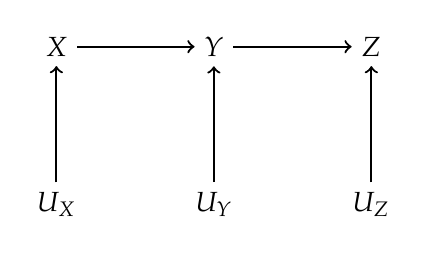
\begin{tikzpicture}
	% Nodes
	\node (X) at (0,0) {$X$};
	\node (Y) at (2,0) {$Y$};
	\node (Z) at (4,0) {$Z$};
	\node (Ux) at (0,-2) {$U_X$};
	\node (Uy) at (2,-2) {$U_Y$};
	\node (Uz) at (4,-2) {$U_Z$};

	% Arrows
	\draw[->,thick] (X) -- (Y);
	\draw[->,thick] (Y) -- (Z);
	\draw[->,thick] (Ux) -- (X);
	\draw[->,thick] (Uy) -- (Y);
	\draw[->,thick] (Uz) -- (Z);
\end{tikzpicture}


\item \textbf{Best guess of the value of Z, given that we observe \( Y = 3 \)}

Given \( Y = 3 \), substituting into the formula \( Z = \frac{Y}{16} + U_Z \) results in \( Z = \frac{3}{16} + U_Z \). Since \( E(U_Z) = 0 \), therefore \( E(Z|Y=3) = \frac{3}{16} + 0 = \frac{3}{16} \).

\item \textbf{Best guess of the value of Z, given that we observe \( X = 3 \)}

Firstly, according to the formula \( Y = \frac{X}{3} + U_Y \) and given \( X = 3 \), we have \( Y = \frac{3}{3} + U_Y = 1 + U_Y \). Then, substituting \( Y = 1 + U_Y \) into \( Z = \frac{Y}{16} + U_Z \) yields \( Z = \frac{(1 + U_Y)}{16} + U_Z \). Since the expected values of \( U_Y \) and \( U_Z \) are 0, \( E(Z|X=3) = E\left(\frac{(1 + U_Y)}{16} + U_Z\right) = \frac{1}{16} + 0 = \frac{1}{16} \).

\item \textbf{Best guess of the value of Z, given that we observe \( X = 1 \) and \( Y = 3 \)}

As \( X \) and \( Y \) values are known, directly using the formula \( Z = \frac{Y}{16} + U_Z \) with \( Y = 3 \) results in \( Z = \frac{3}{16} + U_Z \). Since \( E(U_Z) = 0 \), thus \( E(Z|X=1, Y=3) = \frac{3}{16} \).
\end{enumerate}
  



%------------------------------------------------
\section*{Answer 2}
\begin{enumerate}

\item\begin{itemize}
	\item \( \Pr[\text{Send } 1 | b_i = 1] = \Pr[\text{First coin heads}] \times 1 + \Pr[\text{First coin tails}] \times \Pr[\text{Second coin tails}] \)
	\[
	= \frac{1}{2} \times 1 + \frac{1}{2} \times \frac{1}{2} = \frac{3}{4}
	\]
	
\item \( \Pr[\text{Send } 1 | b_i = 0] = \Pr[\text{First coin tails}] \times \Pr[\text{Second coin tails}] = \frac{1}{2} \times \frac{1}{2} = \frac{1}{4} \)
\end{itemize}


The ratio of these probabilities provides the measure of privacy:
\[ \frac{\Pr[\text{Send } 1 | b_i = 1]}{\Pr[\text{Send } 1 | b_i = 0]} = \frac{3/4}{1/4} = 3 \]
Thus, the privacy parameter \( \epsilon \) is given by:
\[ \epsilon = \ln(3) \]

\item Given the aggregate of \( n \) such \( \tilde{b}_i \) values, the estimator \( \hat{a} \) is formed by adjusting for the bias introduced by the random response mechanism:
\[
\hat{a} = 2 \left( \frac{1}{n} \sum_{i=1}^n \tilde{b}_i - \frac{1}{4} \right)
\]
\[
E[\hat{a}] = 2 \left( E\left[ \frac{1}{n} \sum_{i=1}^n \tilde{b}_i \right] - \frac{1}{4} \right) = 2 \left( \frac{1}{2}a + \frac{1}{4} - \frac{1}{4} \right) = a
\]

\item Finally, the standard deviation of \(\hat{a}\) is:
\[
\text{SD}(\hat{a}) = \sqrt{\text{Var}(\hat{a})} = \sqrt{\frac{1}{n} \left(\frac{1}{4}b_i + \frac{3}{16}\right)} = O\left(\frac{1}{\sqrt{n}}\right)
\]


\item The central model adds Laplace noise to the true mean \(a = \frac{1}{n} \sum_{i=1}^n b_i\) with scale \(\frac{1}{\lambda}\) where \(\lambda = n/\ln(3)\) to achieve \(\ln(3)\)-differential privacy. The variance of the Laplace distribution is given by:
\[
\text{Var}(\text{Laplace}) = \frac{2}{\lambda^2} = \frac{2 \ln(3)^2}{n^2}
\]


So the standard deviation of the estimation error in the central model is:
\[
\text{SD}(\hat{a}_C) = \sqrt{\text{Var}(\hat{a}_C)} = \sqrt{\frac{2 \ln(3)^2}{n^2}} = O\left(\frac{1}{n}\right)
\]

\item To achieve \( \epsilon \)-differential privacy, let \( p \) be the probability of sending 1 when the true bit \( b_i = 1 \), and \( q \) be the probability of sending 1 when \( b_i = 0 \). These probabilities should satisfy:
\[ \frac{p}{q} \leq e^\epsilon \]
\[ \frac{1-q}{1-p} \leq e^\epsilon \]

We set:
\[ p = \frac{e^\epsilon}{1 + e^\epsilon} \]
\[ q = \frac{1}{1 + e^\epsilon} \]

These choices ensure that the privacy guarantee of \( \epsilon \)-differential privacy is met.


The expected value and variance of the randomized response \( \tilde{b}_i \) are given by:
\[ E[\tilde{b}_i] = p \cdot b_i + q \cdot (1 - b_i) \]
\[ \text{Var}(\tilde{b}_i) = E[\tilde{b}_i^2] - (E[\tilde{b}_i])^2 = p(1-p) \cdot b_i + q(1-q) \cdot (1 - b_i) \]

The estimator \( \hat{a} \) for the average \( a \) is:
\[ \hat{a} = \frac{1}{n} \sum_{i=1}^n \tilde{b}_i \]
\[ \text{Var}(\hat{a}) = \frac{1}{n} (p(1-p) \cdot b_i + q(1-q) \cdot (1 - b_i)) \]
\[ \text{SD}(\hat{a}) = \sqrt{\text{Var}(\hat{a})} = \sqrt{\frac{1}{n} (p(1-p) + q(1-q))} \]
\[ \text{SD}(\hat{a}) = \sqrt{\text{Var}(\hat{a})} = \sqrt{\frac{2e^\epsilon}{n(1 + e^\epsilon)^2}}=O\left(\frac{1}{\sqrt{n(\frac{1}{e^\epsilon}+e^\epsilon)}}\right) \] 
Since $\epsilon >0$, $\frac{1}{e^\epsilon} < 1$ and can be ignored. But it stills differ from the result in Q2. It seems works for $ln(\epsilon)-DP$
\end{enumerate}

\section*{Answer 3}

\begin{enumerate}
    \item \textbf{Demographic Parity:}
    First, calculate the proportion of each gender predicted as Yes by each algorithm:
    \begin{itemize}
        \item Proportion of males predicted as Yes by Algorithm 1: $1/4$.
        \item Proportion of males predicted as Yes by Algorithm 2: $3/4$.
        \item Proportion of females predicted as Yes by Algorithm 1: $1/4$.
        \item Proportion of females predicted as Yes by Algorithm 2: $1/4$.
    \end{itemize}
    Algorithm 1 exhibits demographic parity across genders, whereas Algorithm 2 does not, due to different rates for males and females.

    \item \textbf{Equal Opportunity:}
    Calculate the proportion of each gender predicted as Yes when the true label is Yes:
    \begin{itemize}
        \item Proportion of males correctly predicted as Yes by Algorithm 1: $1/3$.
        \item Proportion of males correctly predicted as Yes by Algorithm 2: $1/3$.
        \item Proportion of females correctly predicted as Yes by Algorithm 1: $1/3$.
        \item Proportion of females correctly predicted as Yes by Algorithm 2: $0$.
    \end{itemize}
    Algorithm 1 satisfies equal opportunity since it predicts Yes for both genders at the same rate when the true label is Yes. Algorithm 2 does not satisfy this criterion, especially failing for females.

    \item \textbf{Equalized Odds:}
    Consider the accuracy for each gender across both possible true labels :
    \begin{itemize}
        \item Proportion of males Algorithm 1 correctly predicts Yes: $1/3$, No: $1/3$.
        \item Proportion of males Algorithm 2 correctly predicts Yes: $1/3$, No: $1/3$.
        \item Proportion of females Algorithm 1 correctly predicts Yes: $1/3$, No: $1/3$.
        \item Proportion of females Algorithm 2 correctly predicts Yes: $0$, No: $1/3$.
    \end{itemize}
    Algorithm 1 meets equalized odds as it correctly predicts both outcomes with equal probabilities across genders. Algorithm 2 does not meet this criterion, showing disparity, especially in predicting positive outcomes for females.

\end{enumerate}
\section*{Answer 4}

\begin{enumerate}
    \item 
    \[
    \text{Approval Rate for Group A} = \frac{200}{600} = 33.33\%
    \]

    \item 
    \[
    \text{Approval Rate for Group B} = \frac{50}{400} = 12.5\%
    \]

    \item 
    \[
    \text{Difference in approval rates} = 33.33\% - 12.5\% = 20.83\%
    \]
    Demographic parity is not achieved.

    \item \textbf{Equalized Odds (Assuming Same TPR and FPR for Group B):}
    \[
    \text{TPR for Group B} = 50\%, \quad \text{FPR for Group B} = 20\%
    \]

    \item \begin{itemize}
		\item New approvals needed for Group B: \(0.3333 \times 400 = 133\)
		\item Total approvals if adjusted: \(200 (\text{Group A}) + 133 (\text{Group B}) = 333\)
		\item New overall approval rate: \( \frac{333}{1000} = 33.3\% \)
	\end{itemize}
	Adjusting Group B's approvals to 133 to achieve demographic parity increases the total number of approvals to 333, which exceeds the fixed approval rate of 25\% (250 approvals).
    Decreasing the total number of approvals to 250 to maintain the overall rate makes it impossible to achieve demographic parity and equalized odds without one affecting the other.

\end{enumerate}
%----------------------------------------------------------------------------------------
\section*{Answer 5}
\begin{enumerate}
	\item The Shapley value for player \(i\) is defined as:
\[ \phi_i(v) = \sum_{S \subseteq D\setminus \{i\}} \frac{|S|!(d - |S| - 1)!}{d!} (v(S \cup \{i\}) - v(S)) \]

Since \(i\) is a null player:
\[ v(S \cup \{i\}) - v(S) = 0 \]
for all \(S \subseteq D\setminus \{i\}\).

Substituting into the Shapley value formula, we obtain:
\[ \phi_i(v) = \sum_{S \subseteq D\setminus \{i\}} \frac{|S|!(d - |S| - 1)!}{d!} \cdot 0 = 0 \]

Thus, the Shapley value \(\phi_i(v)\) for a null player \(i\) is 0.
\item Given two cooperative games \(u, v: 2^D \rightarrow \mathbb{R}\) and a game \(w\) defined by \(w(S) = u(S) + v(S)\) for all \(S \subseteq D\)
The Shapley value of player \(i\) in game \(w\) is calculated as follows:
\begin{align*}
	\phi_i(w) &= \sum_{S \subseteq D \setminus \{i\}} \frac{|S|!(d - |S| - 1)!}{d!} \left(w(S \cup \{i\}) - w(S)\right) \\
	&= \sum_{S \subseteq D \setminus \{i\}} \frac{|S|!(d - |S| - 1)!}{d!} \left((u(S \cup \{i\}) + v(S \cup \{i\})) - (u(S) + v(S))\right) \\
	&= \sum_{S \subseteq D \setminus \{i\}} \frac{|S|!(d - |S| - 1)!}{d!} \left((u(S \cup \{i\}) - u(S)) + (v(S \cup \{i\}) - v(S))\right) \\
	&= \phi_i(u) + \phi_i(v)
	\end{align*}

\item 
\begin{align*}
	\sum_{i=1}^d \phi_i(v) &= \sum_{i=1}^d \sum_{S \subseteq D \setminus \{i\}} \frac{|S|!(d - |S| - 1)!}{d!} \left(v(S \cup \{i\}) - v(S)\right) \\
	&= \sum_{S \subseteq D} \sum_{i \in S} \frac{|S|-1|!(d - |S|)!}{d!} \left(v(S) - v(S \setminus \{i\})\right) \\
	&= \sum_{S \subseteq D} \left(v(S) \sum_{i \in S} \frac{|S|-1|!(d - |S|)!}{d!} - v(S \setminus \{i\}) \frac{|S|-1|!(d - |S|)!}{d!} \right) \\
	&= \sum_{S \subseteq D} \frac{1}{d} \left(v(S) - v(\emptyset)\right) \\
	&= v(D) - v(\emptyset)
	\end{align*}

\item \textbf{Null Player Axiom:}
If player \(i\) is a null player, then for any subset \(S\) not containing \(i\), \(v(S \cup \{i\}) = v(S)\). For such a player, 
\[
\phi_i(D \setminus \{j\}) = \phi_i(D) = 0
\]
for any \(j \neq i\). This satisfies the null player condition, as the player's contribution to any subset and thus the whole game is zero.

\textbf{Symmetry Axiom:}
If players \(i\) and \(j\) are symmetric, i.e., \(v(S \cup \{i\}) = v(S \cup \{j\})\) for all \(S \subseteq D \setminus \{i, j\}\), then
\[
\phi_i(D) = \phi_j(D) \quad \text{and} \quad \phi_i(D \setminus \{j\}) = \phi_j(D \setminus \{i\})
\]
This property directly states their Shapley values are equal, confirming the symmetry axiom.

\textbf{Linearity Axiom:}
Given two games \(u\) and \(v\) and their combination \(w(S) = u(S) + v(S)\),
\[
\phi_i(w) = \phi_i(u) + \phi_i(v)
\]
can be derived from linear combinations of values which follow from the additive property of the Shapley value, as each player's marginal contribution to a coalition in a linear combination of games is the sum of their marginal contributions in each game.

\end{enumerate}

\section*{Answer 6}
\begin{enumerate}
\item \begin{itemize}
	\item For player 1:
	\[
	\phi_1(v) = \frac{1}{3!} [(2 - 0) + (5 - 3) + (6 - 4) + (8 - 7)] = \frac{1}{6} [2 + 2 + 2 + 1] = \frac{7}{6}
	\]
	\item For player 2:
	\[
	\phi_2(v) = \frac{1}{3!} [(3 - 0) + (5 - 2) + (7 - 4) + (8 - 6)] = \frac{1}{6} [3 + 3 + 3 + 2] = \frac{11}{6}
	\]
	\item For player 3:
	\[
	\phi_3(v) = \frac{1}{3!} [(4 - 0) + (6 - 2) + (7 - 3) + (8 - 5)] = \frac{1}{6} [4 + 4 + 4 + 3] = \frac{15}{6}
	\]
	\end{itemize}
	\item Since the Shapley values for specific user is constant for different games.
	\begin{itemize}
		\item \(\phi_1(v) = \frac{1}{3}(2 + 2 + 2) = 2\)
		\item \(\phi_2(v) = \frac{1}{3}(3 + 3 + 3) = 3\)
		\item \(\phi_3(v) = \frac{1}{3}(4 + 4 + 4) = 4\)
	\end{itemize}
\item By using the function we calculate the Shapley value table as follows:

\[
\begin{array}{|c|c|c|c|c|}
\hline
\text{Player 1} & \text{Player 2} & \text{Player 3} & \text{Player 4} & \text{Player 5} \\
\hline
-85.5 & -72.5 & -79.5 & 8.0 & 31.5 \\
\hline
\end{array}
\]


Seeing code here\href{q6.py}{Python Code}

\end{enumerate}
\end{document}
